\section{Experiments}
\label{sec:exp}

In this section, we evaluate IGP by implementing it on top of EfficientZero-Multitask (EZ-M)~\citep{liu2026scaling}, and refer to the resulting method as EZ-IGP. We continue to adopt the multi-task training setting. Our experiments aim to answer the following questions: (1) How does EZ-IGP perform compared with established baselines? (2) What is the empirical variance distribution when training with a Gaussian policy? (3) What does the learned policy behavior look like in practical applications? (4) How does performance vary with the number of discretization bins? (5) How does performance change with the number of search rounds? We answer these questions in the following subsections, with additional experimental details and training curves provided in Appendix~\ref{sec:app_curves}.

% \subsection{Experimental Settings}

% \textbf{Benchmarks}. 
% We evaluate EZ-IGP on DMControl~\citep{tassa2018deepmind}, a widely used benchmark for continuous-control reinforcement learning, and HumanoidBench~\citep{sferrazza2024humanoidbench}, a challenging benchmark for whole-body humanoid control that requires coordinating many degrees of freedom under contact-rich dynamics. Compared with the relatively simpler locomotion tasks in DMControl, HumanoidBench includes more demanding tasks such as stair climbing, hurdle traversal, and maze navigation, where existing methods still leave substantial room for improvement.

% Following~\citep{nauman2025bigger} and~\citep{liu2026scaling}, we focus on two challenging task suites: \textit{HB-Hard} and \textit{DMC-Hard}. \textit{HB-Hard} consists of hand-control tasks, including 9 locomotion tasks as well as \texttt{sit-simple}, \texttt{sit-hard}, \texttt{balance-simple}, \texttt{balance-hard}, and \texttt{reach}. \textit{DMC-Hard} contains 7 high-dimensional control tasks: 3 humanoid tasks, \texttt{stand}, \texttt{walk}, and \texttt{run}, and 4 dog tasks, \texttt{stand}, \texttt{walk}, \texttt{run}, and \texttt{trot}. For \textit{HB-Hard}, training is limited to 1 million environment steps without action repeat. For DMControl, training is also limited to 1 million environment steps, with an action repeat of 2.

% \textbf{Baselines}. 
% On HumanoidBench, we compare EZ-IGP against established baselines spanning both single-task (ST) and multi-task (MT) settings, as well as model-free (MF) and model-based (MB) methods. The main baselines include \textbf{TD-MPC2} (ST, MB)~\citep{hansen2023td}, \textbf{MH-SAC} (MT, MF)~\citep{yang2020multi}, \textbf{BRC} (MT, MF)~\citep{nauman2025bigger}, and \textbf{EZ-M} (MT, MB)~\citep{liu2026scaling}. On DMControl, we compare EZ-IGP with \textbf{TD-MPC2} (ST, MB) and \textbf{EZ-M} (MT, MB). EZ-IGP uses the same network architectures and loss objectives as EZ-M, but replaces the Gaussian policy with our iteratively refined factorized policy. Baseline scores are taken directly from published results when available; otherwise, we report results obtained by re-evaluating the official implementations. We also provide hyperparameter details in Appendix \ref{app:hyperparameters}.

% \textbf{Evaluation Metrics}. 
% To assess aggregate performance, we report normalized scores computed as described in Appendix~\ref{app:score-norm}. In addition, we provide full training curves of original returns against environment steps in Figure~\ref{fig:dmc-unnorm-curves} and Figure~\ref{fig:hb-unnorm-curves} in Appendix~\ref{sec:app_curves}.

\subsection{Experimental Settings}

\textbf{Benchmarks}. 
We evaluate EZ-IGP on two challenging continuous-control benchmarks: DMControl~\citep{tassa2018deepmind} and HumanoidBench~\citep{sferrazza2024humanoidbench}. Following~\citep{nauman2025bigger,liu2026scaling}, we focus on \textit{DMC-Hard} and \textit{HB-Hard}. \textit{DMC-Hard} includes 7 high-dimensional locomotion tasks: humanoid \texttt{stand}, \texttt{walk}, and \texttt{run}, and dog \texttt{stand}, \texttt{walk}, \texttt{run}, and \texttt{trot}. \textit{HB-Hard} consists of hand-control humanoid tasks, including 9 locomotion tasks as well as \texttt{sit-simple}, \texttt{sit-hard}, \texttt{balance-simple}, \texttt{balance-hard}, and \texttt{reach}. We train all methods for 1 million environment steps; DMControl uses an action repeat of 2, while HumanoidBench uses no action repeat.

\textbf{Baselines}. 
On HumanoidBench, we compare EZ-IGP with representative single-task and multi-task baselines, including TD-MPC2~\citep{hansen2023td}, MH-SAC~\citep{yang2020multi}, BRC~\citep{nauman2025bigger}, and EZ-M~\citep{liu2026scaling}. On DMControl, we compare against TD-MPC2 and EZ-M. EZ-IGP follows the same architectures and training objectives as EZ-M, but replaces its Gaussian policy with our iteratively refined factorized policy. Baseline scores are taken from published results when available, and otherwise from re-evaluations of official implementations. Hyperparameter details are provided in Appendix~\ref{app:hyperparameters}.

\textbf{Evaluation Metrics}. 
We report normalized aggregate scores as described in Appendix~\ref{app:score-norm}, and provide full training curves with original returns in Appendix~\ref{sec:app_curves}.


\subsection{Overall Performance}

\textbf{Main results on DMControl dog and humanoid tasks}. Figure \ref{fig:dmc-unnorm-curves} and Table \ref{tab:dmc_scores_with_igp} show results on the DMControl dog and humanoid locomotion tasks; the full per-task score table is placed in the appendix to preserve the nine-page main-text budget. EZ-IGP consistently outperforms or matches all baselines across the seven environments. The improvement is especially pronounced on the dog tasks. On the four dog tasks, EZ-IGP learns faster and achieves the highest \textcolor{blue}{reported per-seed peak scores}. This indicates that the proposed factorized iterative policy is not only effective for dexterous manipulation-like tasks, but also transfers well to high-dimensional locomotion domains with complex contact dynamics.

The same pattern appears on the humanoid tasks: EZ-IGP obtains the best \textcolor{blue}{reported peak performance} and generally shows stronger sample efficiency than BRC, BRC-ST, TD-MPC2, and EZ-M, with especially clear gains on \texttt{humanoid-walk} and \texttt{humanoid-run}, where several baselines plateau at lower scores. This suggests that iterative action refinement becomes more beneficial as tasks require more accurate long-horizon coordination.

Taken together, these results show that EZ-IGP provides a simple but effective alternative to continuous Gaussian policy parameterization by factorizing the action space into discrete per-dimension choices and improving candidate actions through iterative refinement. The resulting policy achieves strong sample efficiency, competitive stability, and state-of-the-art or near state-of-the-art performance across both HumanoidBench and DMControl high-dimensional control tasks.


\paragraph{Main results on HumanoidBench.}
Figure~\ref{fig:hb-unnorm-curves} reports learning curves on the high-dimensional HumanoidBench tasks, while full per-task scores and uncertainty are provided in Table~\ref{tab:humanoidbench_hard}. Overall, EZ-IGP achieves strong and consistent performance across a broad set of challenging dexterous-control environments. Compared with EZ-M, EZ-IGP often learns substantially faster and reaches higher final returns, especially on tasks such as \texttt{h1hand-walk}, \texttt{h1hand-run}, \texttt{h1hand-pole}, and \texttt{h1hand-maze}. These tasks require coordinated control over many action dimensions, where Gaussian policy optimization can be sensitive to variance and exploration scale; in contrast, EZ-IGP provides a structured factorized action proposal and further improves selected actions through iterative planning.

The advantage of EZ-IGP is particularly clear in tasks where successful behavior requires precise multi-dimensional coordination rather than simply discovering a coarse locomotion pattern. For example, in \texttt{h1hand-run} and \texttt{h1hand-pole}, EZ-IGP rapidly improves after the early training phase and eventually reaches a much higher score than BRC, BRC-ST, and TD-MPC2. On \texttt{h1hand-reach}, EZ-M achieves the highest score, while EZ-IGP remains stronger than TD-MPC2, BRC, and BRC-ST.

\textcolor{blue}{EZ-IGP trails the strongest baseline on five HB-Hard tasks. Capacity is a substantial confound: reducing BRC from approximately 1B to 16M parameters lowers its normalized score from $0.576$ to $0.487\pm0.038$, while EZ-IGP reaches $0.787$ at 16M parameters. BRC-16M nevertheless remains stronger on the sitting tasks, indicating a residual task-specific gap whose cause is not isolated by these comparisons.}

\subsection{Policy variance comparisons}
\label{sec:exp:variance}

% \begin{wrapfigure}{r}{0.5\textwidth}
%     \centering
%     \vspace{-10pt}
%     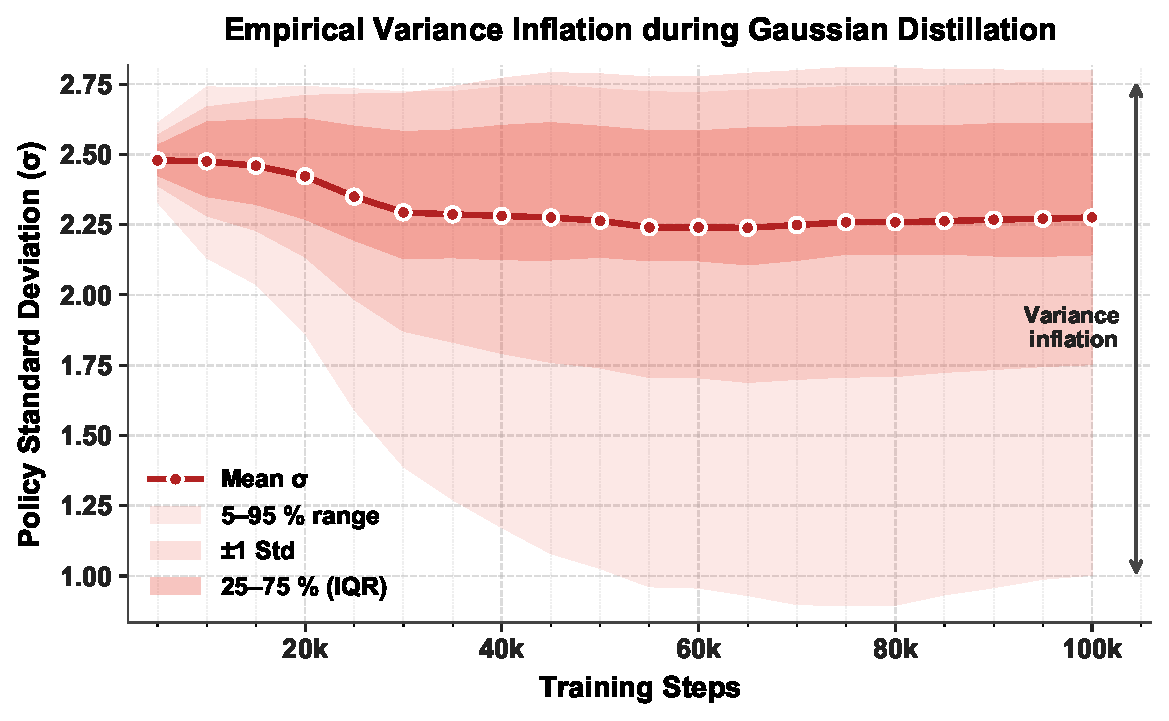
\includegraphics[width=0.5\textwidth]{figs/variance_line.pdf}
%     \caption{\textbf{Persistent variance inflation in Gaussian distillation.} The Gaussian policy standard deviation ($\sigma$) quickly rises and remains high, with the solid line showing the median and shaded regions showing the interquartile and 5--95\% ranges.}
%     \label{fig:var_dist}
%     \vspace{-10pt}
% \end{wrapfigure}

\begin{figure}[t]
    % \vskip -.6cm
    \centering
    % 第一张图 (a)
    \begin{minipage}[t]{0.49\textwidth}
        \centering
        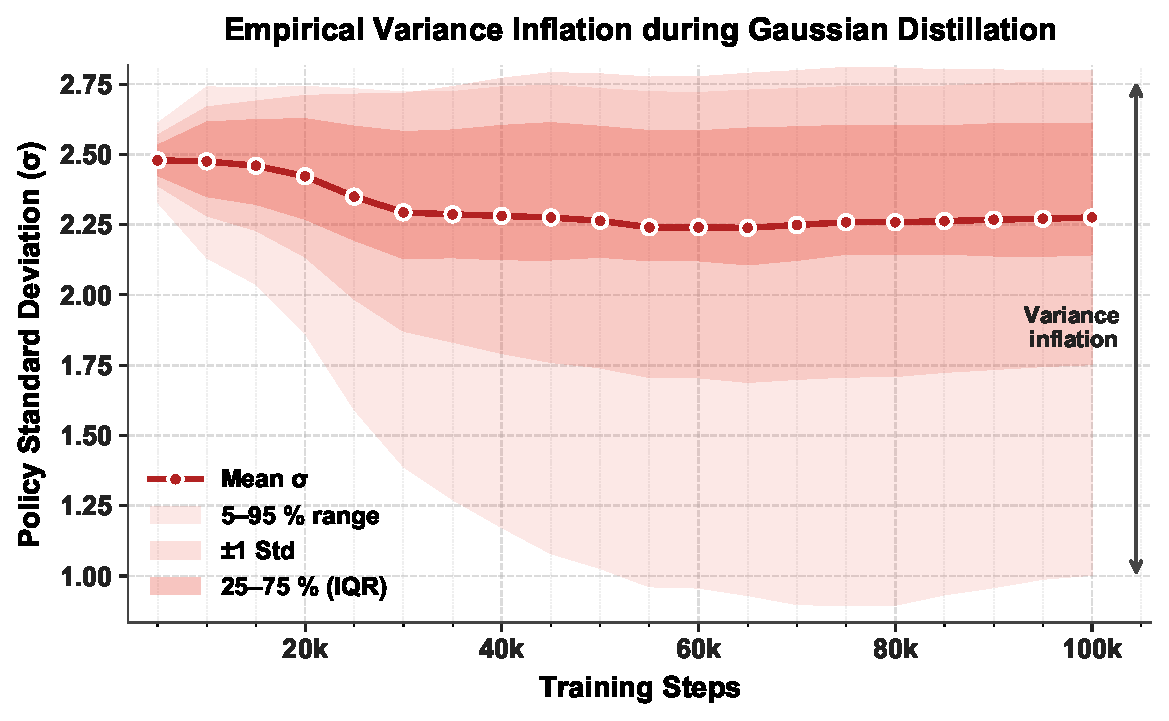
\includegraphics[width=\textwidth]{figs/variance_line.pdf}
        \vspace{0.1cm} % 稍微空一点，让 (a) 不要太贴图
        \centerline{(a) Policy variance distribution in Gaussian distillation.}
    \end{minipage}% <-- 这个 % 依然保留，防止意外换行
    \hfill
    % 第二张图 (b)
    \begin{minipage}[t]{0.49\textwidth}
        \centering
        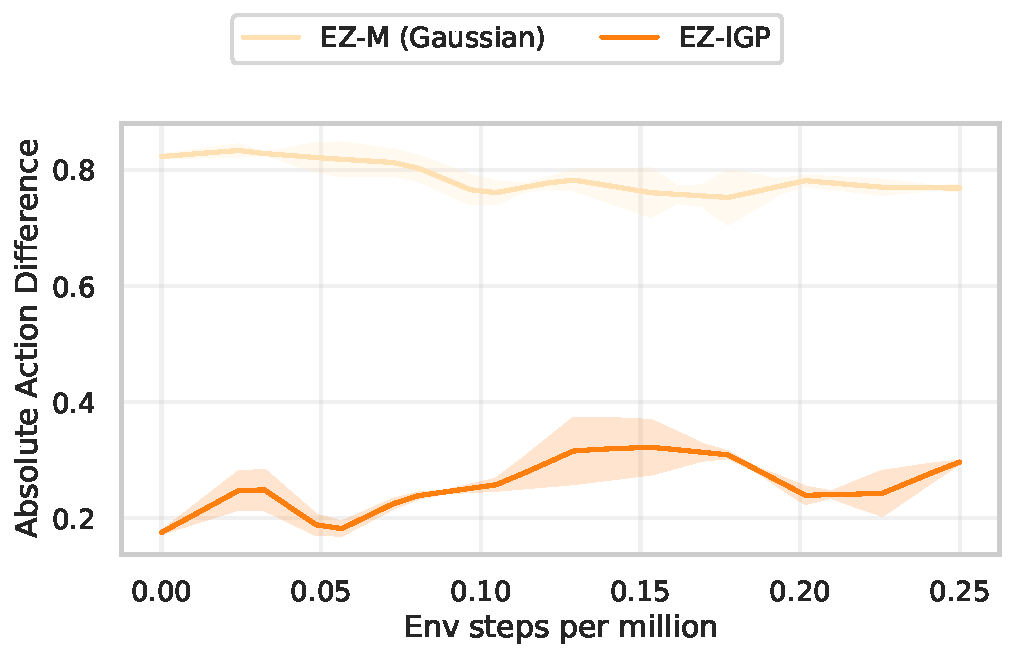
\includegraphics[width=\textwidth]{figs/action_diff.pdf}
        \vspace{0.1cm}
        \centerline{(b) Average $|\Delta a|$ across three humanoid tasks.}
    \end{minipage}
    
    \caption{\textbf{Temporal variance comparisons.} \textbf{(a)} \textcolor{blue}{The Gaussian policy standard deviation ($\sigma$) rises early and remains elevated throughout the observed training horizon}; the solid line shows the median and shaded regions show the interquartile and 5--95\% ranges. \textbf{(b)} The Gaussian policy maintains much larger action changes across adjacent timesteps during evaluation, whereas EZ-IGP consistently produces smaller action differences, suggesting smoother and less jittery control behavior.}
    \label{fig:var_comp}
    \vskip -.2cm
\end{figure}



% Figure~\ref{fig:var_dist} shows that Gaussian policy distillation leads to persistent variance inflation. Instead of gradually reducing uncertainty as training progresses, the learned policy standard deviation quickly rises to a large value and remains high for the rest of training. The median $\sigma$ stabilizes around a high level, and both the interquartile range and the 5--95\% range suggest that this behavior is not caused by a few outlier dimensions or tasks. This indicates that the Gaussian policy does not naturally collapse toward a sharp action distribution after distillation; rather, it maintains substantial stochasticity even after many training steps. Such inflated variance can weaken action precision and make the distilled policy less effective for continuous control. In contrast, our proposed IGP achieves lower temporal variance on action sequences, providing a better chance for future real-world deployment. The qualitative comparison videos can be accessed at \href{https://mellifluous-marzipan-a1cb45.netlify.app/}{this anonymous website}.

\textcolor{blue}{Figure~\ref{fig:var_comp}(a) empirically demonstrates the sustained training-time consequence of the update-level mechanism in Proposition~\ref{prop:gaussian_var_inflation}: the standard deviation rises early and remains high throughout the observed training horizon, including its final stage.} The median $\sigma$ stabilizes around a high level, and both the interquartile range and the 5--95\% range suggest that this behavior is not caused by a few outlier dimensions or tasks. Figure~\ref{fig:var_comp}(b) further shows that this elevated variance is reflected in the realized policy behavior: EZ-M with a Gaussian policy produces much larger temporal action differences, while EZ-IGP maintains substantially smoother action sequences. Such action fluctuations can weaken control precision and lead to jittery behaviors in continuous-control tasks. The qualitative comparison videos can be accessed at \href{https://mellifluous-marzipan-a1cb45.netlify.app/}{this anonymous website}.

\paragraph{\textcolor{blue}{Refinement-matched Gaussian control.}}
\textcolor{blue}{With the same backbone, search budget, and two refinement rounds, EZ-IGP improves all three DMC humanoid tasks by 139--150 points over a matched Gaussian proposal (Table~\ref{tab:matched_gaussian_refine}). The Gaussian scale remains elevated late in training, including when distilling a search-weighted mixture of candidates; thus neither refinement nor distributing target mass removes the observed scale pressure.}


\subsection{Ablation Study}

Figure~\ref{fig:ablations} and Table~\ref{tab:hb_hard_vr_sweep} support
$V=31$, $R=2$ as a practical rather than universal performance--computation
trade-off: coarse bins hurt, two rounds improve over one, and four rounds add
little or degrade some tasks. Table~\ref{tab:simulation_budget} further shows
monotonic degradation under smaller search budgets, reflecting reduced
candidate coverage and ranking quality.

% \begin{wrapfigure}{r}{0.6\textwidth}
%     \centering
%     \vspace{-10pt}
%     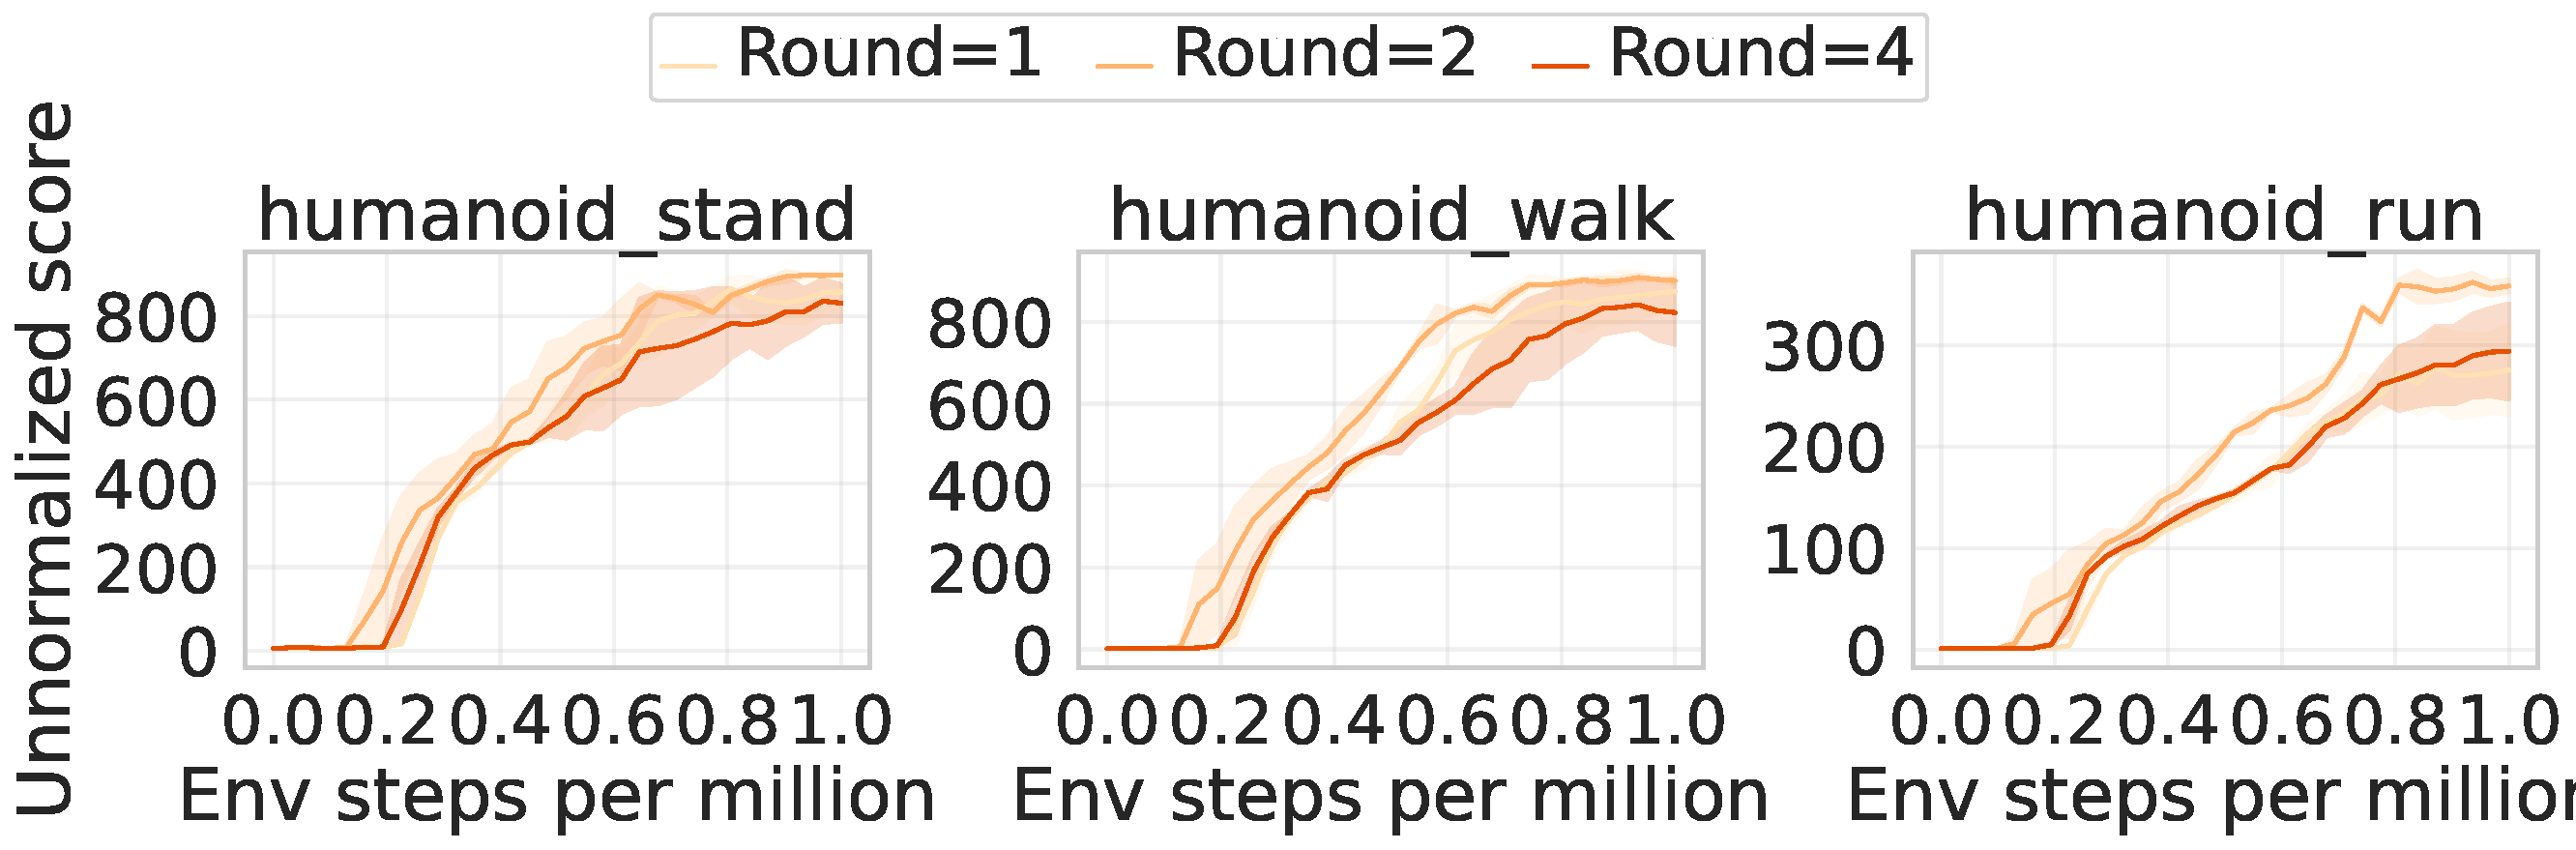
\includegraphics[width=0.58\textwidth]{figs/Round_ablation.pdf}
%     \caption{\textbf{Effect of the number of refinement rounds.}
% We ablate the number of iterative search-refinement rounds on three HumanoidBench locomotion tasks. A moderate number of rounds generally improves performance, but using too many rounds (e.g., 4) leads to worse results, especially on \texttt{humanoid\_walk} and \texttt{humanoid\_run}. This suggests that excessive refinement can make the policy overly deterministic, reducing effective exploration during training.}
%     \label{fig:round_ablation}
%     \vspace{-10pt}
% \end{wrapfigure}
